% fig_coord_architecture.tex
% TR-35: Complete IBR protection architecture block diagram
% Shows all five protection functions and their inputs/outputs
% as a layered defensive stack

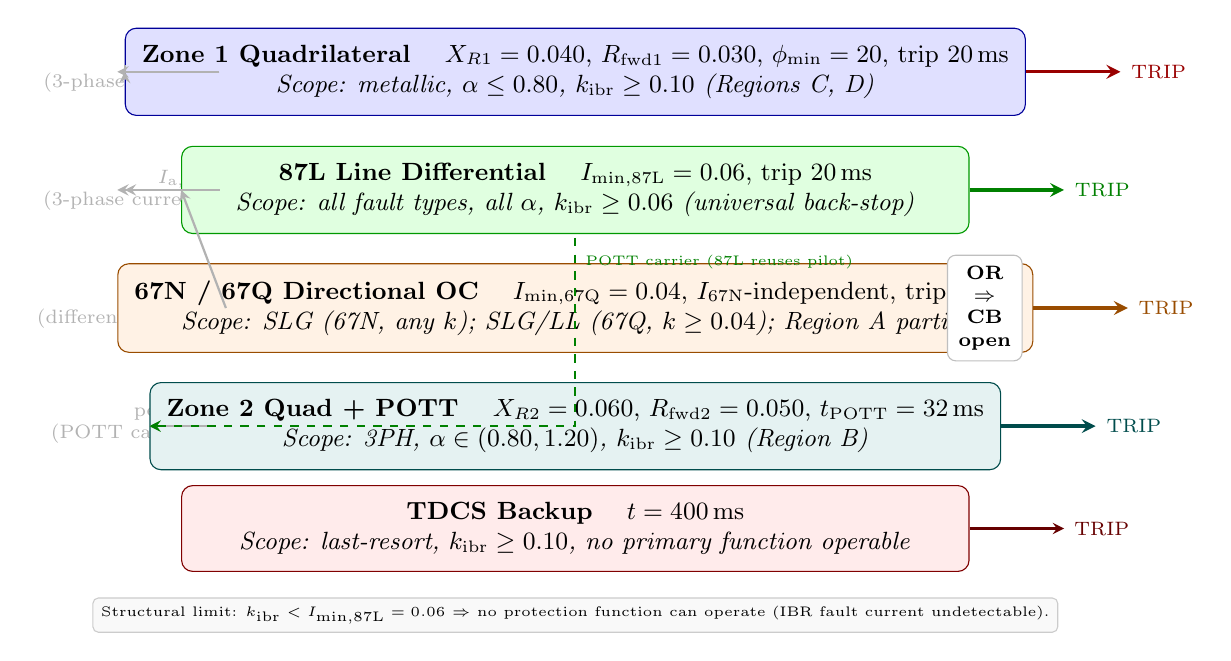
\begin{tikzpicture}[
  every node/.style = {font=\small},
  layer/.style = {draw, rounded corners=4pt, inner sep=6pt,
                  minimum width=10.0cm, minimum height=1.0cm,
                  align=center},
  inputarr/.style = {->, >=stealth, thick, gray!60},
  note/.style = {font=\tiny, text=gray!70, align=right},
]

%% ── Input signals (left side) ────────────────────────────────────────────────
\node[font=\scriptsize, align=right, gray!60] (inV) at (-2.2, 5.5)
  {$V_\mathrm{a,b,c}$\\(3-phase voltage)};
\node[font=\scriptsize, align=right, gray!60] (inI) at (-2.2, 4.0)
  {$I_\mathrm{a,b,c}$\\(3-phase current)};
\node[font=\scriptsize, align=right, gray!60] (inDiff) at (-2.2, 2.5)
  {$I_\mathrm{diff}$\\(differential, pilot)};
\node[font=\scriptsize, align=right, gray!60] (inPerm) at (-2.2, 1.0)
  {$\mathrm{perm}_\mathrm{rx}$\\(POTT carrier)};

%% ── Layer 1: Zone 1 Quadrilateral ────────────────────────────────────────────
\node[layer, fill=blue!12, draw=blue!60!black] (L1) at (3.5, 5.5)
  {\textbf{Zone 1 Quadrilateral} \quad $X_{R1}=0.040$, $R_\mathrm{fwd1}=0.030$,
   $\phi_\mathrm{min}=20°$, trip 20\,ms\\
   \textit{Scope: metallic, $\alpha\leq0.80$, $k_\mathrm{ibr}\geq0.10$ (Regions C, D)}};

%% ── Layer 2: 87L Differential ────────────────────────────────────────────────
\node[layer, fill=green!12, draw=green!60!black] (L2) at (3.5, 4.0)
  {\textbf{87L Line Differential} \quad $I_\mathrm{min,87L}=0.06$, trip 20\,ms\\
   \textit{Scope: all fault types, all $\alpha$, $k_\mathrm{ibr}\geq0.06$ (universal back-stop)}};

%% ── Layer 3: 67N/67Q Directional ─────────────────────────────────────────────
\node[layer, fill=orange!10, draw=orange!60!black] (L3) at (3.5, 2.5)
  {\textbf{67N / 67Q Directional OC} \quad $I_\mathrm{min,67Q}=0.04$,
   $I_\mathrm{67N}$-independent, trip 30\,ms\\
   \textit{Scope: SLG (67N, any $k$); SLG/LL (67Q, $k\geq0.04$); Region~A partial}};

%% ── Layer 4: Zone 2 / POTT ───────────────────────────────────────────────────
\node[layer, fill=teal!10, draw=teal!60!black] (L4) at (3.5, 1.0)
  {\textbf{Zone 2 Quad + POTT} \quad $X_{R2}=0.060$, $R_\mathrm{fwd2}=0.050$,
   $t_\mathrm{POTT}=32$\,ms\\
   \textit{Scope: 3PH, $\alpha\in(0.80,1.20)$, $k_\mathrm{ibr}\geq0.10$ (Region~B)}};

%% ── Layer 5: TDCS Backup ─────────────────────────────────────────────────────
\node[layer, fill=red!8, draw=red!50!black] (L5) at (3.5, -0.3)
  {\textbf{TDCS Backup} \quad $t=400$\,ms\\
   \textit{Scope: last-resort, $k_\mathrm{ibr}\geq0.10$, no primary function operable}};

%% ── TRIP output (right side) ─────────────────────────────────────────────────
\draw[->, >=stealth, very thick, red!60!black]
  (L1.east) -- ++(1.2,0) node[right, red!60!black, font=\scriptsize] {TRIP};
\draw[->, >=stealth, very thick, green!50!black]
  (L2.east) -- ++(1.2,0) node[right, green!50!black, font=\scriptsize] {TRIP};
\draw[->, >=stealth, very thick, orange!60!black]
  (L3.east) -- ++(1.2,0) node[right, orange!60!black, font=\scriptsize] {TRIP};
\draw[->, >=stealth, very thick, teal!60!black]
  (L4.east) -- ++(1.2,0) node[right, teal!60!black, font=\scriptsize] {TRIP};
\draw[->, >=stealth, thick, red!40!black]
  (L5.east) -- ++(1.2,0) node[right, red!40!black, font=\scriptsize] {TRIP};

%% ── Input arrows ─────────────────────────────────────────────────────────────
\draw[inputarr] (inV.east) -- (L1.west |- inV) -- (L1.west);
\draw[inputarr] (inV.east) -- (L3.west |- inV);
\draw[inputarr] (inI.east) -- (L1.west |- inI);
\draw[inputarr] (inI.east) -- (L3.west |- inI);
\draw[inputarr] (inDiff.east) -- (L2.west);
\draw[inputarr] (inPerm.east) -- (L4.west);

%% ── 87L feeds POTT carrier ───────────────────────────────────────────────────
\draw[->, >=stealth, thick, green!50!black, dashed]
  (L2.south) ++(0,-0.05) -- ++(0,-0.30)
  node[right, green!50!black, font=\tiny] {POTT carrier (87L reuses pilot)}
  |- (L4.west);

%% ── "OR" logic ────────────────────────────────────────────────────────────────
\node[draw=gray!50, fill=white, rounded corners=3pt,
      font=\scriptsize\bfseries, inner sep=4pt, align=center]
  at (8.7, 2.5) {OR\\$\Rightarrow$\\CB\\open};

%% ── Structural limit annotation ───────────────────────────────────────────────
\node[draw=gray!40, fill=gray!5, rounded corners=2pt,
      font=\tiny, inner sep=3pt, align=center]
  at (3.5, -1.4)
  {Structural limit: $k_\mathrm{ibr} < I_\mathrm{min,87L}=0.06$ $\Rightarrow$
   no protection function can operate (IBR fault current undetectable).};

\end{tikzpicture}
